%================================================
% PACKAGES AND THEMES
%================================================
\documentclass[t,aspectratio=169,xcolor=dvipsnames]{beamer}

\usetheme{SimplePlusAIC}

\usepackage{graphicx}
\usepackage{booktabs}
\usepackage{svg}
\usepackage{tcolorbox}
\usepackage{tikz}
\usetikzlibrary{shapes.geometric, arrows, positioning, fit, calc}
\usepackage{makecell}
\usepackage{listings}

\newcommand*{\defeq}{\stackrel{\text{def}}{=}}
\usepackage{setspace}
\usepackage[T1]{fontenc}
\usepackage{helvet}
\usepackage{amsmath}
\usepackage{ragged2e}
\usepackage{gensymb}

\usepackage[svgnames,table]{xcolor}
\arrayrulecolor{black}
\setlength{\arrayrulewidth}{0.20mm}
\renewcommand{\arraystretch}{1.35}

\newcommand{\tem}[1]{\textbf{\textcolor{red}{#1}}}

% Listings configuration
\lstset{
    basicstyle=\ttfamily\small,
    breaklines=true,
    columns=fullflexible,
    frame=none
}

%================================================
% TITLE PAGE
%================================================
\title[Paging and Address Translation]{Memory Management 3: Paging}
\subtitle{Week 7: Perhitungan Alamat dengan Basis 2}
\author[informatika-itera.github.io/os]{informatika-itera.github.io/os}
\institute[ITERA]{Program Studi Teknik Informatika \\ Institut Teknologi Sumatera}
\date{\textcolor{nyublue}{2026}}

%================================================
% BEGIN DOCUMENT
%================================================
\begin{document}

\begin{frame}
    \titlepage
\end{frame}

\begin{frame}
    \frametitle{OUTLINE}
    \framesubtitle{Peta materi pertemuan ini}
    \small
    \begin{spacing}{1.15}
        \tableofcontents
    \end{spacing}
\end{frame}

\begin{frame}
    \frametitle{Capaian Pembelajaran}
    \framesubtitle{Tujuan setelah pertemuan selesai}
    \small
    \begin{enumerate}
        \item Memahami konsep dasar page, frame, dan page table.
        \item Menghitung jumlah bit untuk page number, offset, dan frame number berdasarkan ukuran memori (basis 2).
        \item Melakukan translasi alamat logis ke alamat fisik dengan rumus dasar.
        \item Memvalidasi alamat logis dan mendeteksi page fault.
        \item Menerapkan konsep paging pada sistem memori berskala besar (MB, GB).
    \end{enumerate}
    \begin{exampleblock}{Fokus Kelas Ini}
        Kita fokus pada \tem{perhitungan biner} dan \tem{translasi alamat} step-by-step dengan banyak latihan praktis.
    \end{exampleblock}
\end{frame}

\section{Konsep Dasar Paging}

\begin{frame}
    \frametitle{Apa Itu Paging?}
    \framesubtitle{Teknik manajemen memori modern}
    \small
    \begin{block}{Definisi}
        Paging adalah teknik yang memungkinkan alamat fisik memori \\tem{tidak harus bersambungan} (noncontiguous) saat mengalokasikan ruang untuk proses.
    \end{block}

    \vspace{0.2cm}
    \textbf{Tiga elemen kunci:}
    \begin{itemize}
        \item \textbf{Page:} Unit memori logis (address space proses) berukuran tetap.
        \item \textbf{Frame:} Unit memori fisik (RAM) berukuran sama dengan page.
        \item \textbf{Page Table:} Struktur data yang memetakan page $\rightarrow$ frame.
    \end{itemize}

    \vspace{0.2cm}
    \begin{alertblock}{Penting}
        \textbf{Ukuran page dan frame {\em harus sama}} untuk memastikan mapping berjalan benar!
    \end{alertblock}
\end{frame}

\begin{frame}
    \frametitle{Page vs Frame: Visualisasi}
    \framesubtitle{Memori logis vs memori fisik}
    \small
    \begin{columns}[T]
        \column{0.45\textwidth}
        \textbf{Memori Logis (Proses)}
        \begin{itemize}
            \item Program melihat memorinya linear dan bersambung.
            \item Dibagi menjadi \textit{page} dengan ukuran tetap.
            \item Contoh: 4 KB/page, 8 KB/page.
        \end{itemize}

        \column{0.45\textwidth}
        \textbf{Memori Fisik (RAM)}
        \begin{itemize}
            \item RAM dibagi menjadi \textit{frame} dengan ukuran sama.
            \item Frame dapat dialokasikan secara noncontiguous.
            \item Page dapat berada di mana saja di RAM.
        \end{itemize}
    \end{columns}

    \vspace{0.2cm}
    \centering
    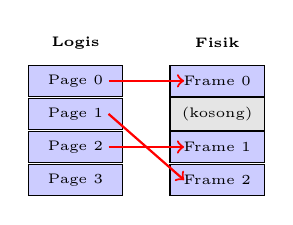
\begin{tikzpicture}[scale=0.6]
        % Logical Memory
        \node[font=\tiny\bfseries] at (-1.5, 4.0) {Logis};
        \foreach \i in {0,1,2,3} {
            \node[draw, rectangle, minimum width=1.2cm, minimum height=0.4cm, fill=blue!20, font=\tiny] at (-1.5, 3.2 - 0.7*\i) {Page \i};
        }

        % Physical Memory
        \node[font=\tiny\bfseries] at (1.5, 4.0) {Fisik};
        \node[draw, rectangle, minimum width=1.2cm, minimum height=0.4cm, fill=blue!20, font=\tiny] at (1.5, 3.2) {Frame 0};
        \node[draw, rectangle, minimum width=1.2cm, minimum height=0.4cm, fill=gray!20, font=\tiny] at (1.5, 2.5) {(kosong)};
        \node[draw, rectangle, minimum width=1.2cm, minimum height=0.4cm, fill=blue!20, font=\tiny] at (1.5, 1.8) {Frame 1};
        \node[draw, rectangle, minimum width=1.2cm, minimum height=0.4cm, fill=blue!20, font=\tiny] at (1.5, 1.1) {Frame 2};

        % Arrows
        \draw[->, red, thick] (-0.8, 3.2) -- (0.8, 3.2);
        \draw[->, red, thick] (-0.8, 2.5) -- (0.8, 1.1);
        \draw[->, red, thick] (-0.8, 1.8) -- (0.8, 1.8);
    \end{tikzpicture}
\end{frame}

\begin{frame}
    \frametitle{Page Table: Mapping Page ke Frame}
    \framesubtitle{Struktur data penting dalam paging}
    \small
    \begin{columns}[T]
        \column{0.50\textwidth}
        \begin{block}{Page Table Format}
            \begin{tabular}{|c|c|c|}
                \hline
                \textbf{Page \#} & \textbf{Frame \#} & \textbf{Valid Bit} \\
                \hline
                0 & 2 & 1 \\
                \hline
                1 & 5 & 1 \\
                \hline
                2 & 0 & 1 \\
                \hline
                3 & 7 & 1 \\
                \hline
                4 & - & 0 \\
                \hline
            \end{tabular}
        \end{block}

        \column{0.45\textwidth}
        \begin{alertblock}{Isi Page Table}
            \begin{itemize}
                \item Entry ke-$i$ menyimpan frame number tempat page-$i$ berada.
                \item Valid bit: 1 = page ada di memori, 0 = page tidak valid.
                \item OS dan MMU menggunakan ini setiap akses memori.
            \end{itemize}
        \end{alertblock}
    \end{columns}
\end{frame}

\section{Perhitungan Bit dan Bilangan Basis 2}

\begin{frame}
    \frametitle{Konsep: Memerlukan Berapa Bit?}
    \framesubtitle{Hubungan antara ukuran dan jumlah bit}
    \small
    \begin{block}{Rumus Dasar}
        Jika ada $n$ item (page, frame, lokasi), maka memerlukan \textbf{$k$ bit} di mana $2^k \geq n$.

        Dengan kata lain: $k = \lceil \log_2 n \rceil$
    \end{block}

    \vspace{0.2cm}
    \textbf{Contoh:}
    \begin{itemize}
        \item 4 page memerlukan $\lceil \log_2 4 \rceil = 2$ bit (karena $2^2 = 4$).
        \item 8 page memerlukan $\lceil \log_2 8 \rceil = 3$ bit (karena $2^3 = 8$).
        \item 256 byte page memerlukan $\lceil \log_2 256 \rceil = 8$ bit offset (karena $2^8 = 256$).
    \end{itemize}

    \begin{exampleblock}{Tip Praktis}
        \textbf{Offset (dalam bytes) = 2$^k$ $\Rightarrow$ memerlukan $k$ bit offset}
    \end{exampleblock}
\end{frame}

\begin{frame}
    \frametitle{Tabel Referensi Basis 2}
    \framesubtitle{Standar yang sering muncul}
    \small
    \begin{table}[]
        \centering
        \begin{tabular}{|c|c|c|c|c|}
            \hline
            \textbf{Bit} & \textbf{Kombinasi} & \textbf{Byte/Item} & \textbf{Contoh} \\
            \hline
            1 bit & $2^1$ & 2 & 2 item \\
            \hline
            2 bit & $2^2$ & 4 & 4 page \\
            \hline
            3 bit & $2^3$ & 8 & 8 frame \\
            \hline
            4 bit & $2^4$ & 16 & 16 byte \\
            \hline
            8 bit & $2^8$ & 256 & 256 byte (0.25 KB) \\
            \hline
            10 bit & $2^{10}$ & 1024 & 1 KB \\
            \hline
            12 bit & $2^{12}$ & 4096 & 4 KB (page standar) \\
            \hline
            20 bit & $2^{20}$ & 1.048.576 & 1 MB \\
            \hline
            30 bit & $2^{30}$ & 1.073.741.824 & 1 GB \\
            \hline
        \end{tabular}
    \end{table}
\end{frame}

\begin{frame}
    \frametitle{Tangga Satuan Memory: 2$^{10}$ Ladder}
    \framesubtitle{Hubungan antara Byte, KB, MB, GB, TB}
    \small

    \begin{center}
        \begin{tabular}{|c|c|c|}
            \hline
            \textbf{Satuan} & \textbf{Nilai} & \textbf{Arti} \\
            \hline
            1 B (Byte) & $2^0$ & 1 byte \\
            \hline
            1 KB (Kilobyte) & $2^{10}$ & 1024 byte \\
            \hline
            1 MB (Megabyte) & $2^{20}$ & 1024 KB = 1.048.576 byte \\
            \hline
            1 GB (Gigabyte) & $2^{30}$ & 1024 MB = 1.073.741.824 byte \\
            \hline
            1 TB (Terabyte) & $2^{40}$ & 1024 GB \\
            \hline
        \end{tabular}
    \end{center}

    \vspace{0.3cm}
    \begin{alertblock}{Pola Kunci}
        Setiap level naik/turun, kalikan/bagi dengan \textbf{$2^{10}$ = 1024} (bukan 1000!).
        \begin{itemize}
            \item Naik: 1 MB = 1024 KB (kalikan dengan 1024)
            \item Turun: 1 MB = 1 $\times$ $2^{20}$ byte (kalikan dengan $2^{20}$)
        \end{itemize}
    \end{alertblock}
\end{frame}

\begin{frame}
    \frametitle{Perkalian dalam Basis 2}
    \framesubtitle{Pangkat ditambahkan saat dikalikan}
    \scriptsize

    \begin{block}{Aturan Dasar Eksponen}
        \[
        2^a \times 2^b = 2^{a+b}
        \]
    \end{block}

    \vspace{0.2cm}
    \textbf{Contoh 1: Konversi byte ke KB}
    \begin{itemize}
        \item Diketahui: 2048 byte
        \item Hitungan: $2048 \div 2^{10} = 2^{11} \div 2^{10} = 2^{11-10} = 2^1 = 2$ KB
        \item Atau: $2048 = 2 \times 1024 = 2$ KB
    \end{itemize}

    \vspace{0.2cm}
    \textbf{Contoh 2: Konversi KB ke byte}
    \begin{itemize}
        \item Diketahui: 8 KB
        \item Hitungan: $8 \times 2^{10} = 2^3 \times 2^{10} = 2^{3+10} = 2^{13} = 8192$ byte
    \end{itemize}

    \vspace{0.2cm}
    \textbf{Contoh 3: Konversi MB ke byte}
    \begin{itemize}
        \item Diketahui: 4 MB
        \item Hitungan: $4 \times 2^{20} = 2^2 \times 2^{20} = 2^{22} = 4.194.304$ byte
    \end{itemize}
\end{frame}

\begin{frame}
    \frametitle{Pembagian dalam Basis 2}
    \framesubtitle{Pangkat dikurangkan saat dibagi}
    \scriptsize

    \begin{block}{Aturan Dasar Eksponen}
        \[
        \frac{2^a}{2^b} = 2^{a-b}
        \]
    \end{block}

    \vspace{0.2cm}
    \textbf{Contoh 1: Berapa banyak KB dalam 4096 byte?}
    \begin{itemize}
        \item Hitungan: $\frac{4096}{1024} = \frac{2^{12}}{2^{10}} = 2^{12-10} = 2^2 = 4$ KB
    \end{itemize}

    \vspace{0.2cm}
    \textbf{Contoh 2: Berapa banyak MB dalam 1 GB?}
    \begin{itemize}
        \item Hitungan: $\frac{2^{30}}{2^{20}} = 2^{30-20} = 2^{10} = 1024$ MB
    \end{itemize}

    \vspace{0.2cm}
    \textbf{Contoh 3: Berapa banyak frame 4 KB dalam 256 MB?}
    \begin{itemize}
        \item 256 MB = $2^8 \times 2^{20} = 2^{28}$ byte
        \item Jumlah frame = $\frac{2^{28}}{2^{12}} = 2^{28-12} = 2^{16} = 65.536$ frame
    \end{itemize}
\end{frame}

\begin{frame}
    \frametitle{Latihan: Konversi Satuan Memory}
    \framesubtitle{Gunakan pangkat 2 untuk mempermudah}
    \small

    \begin{columns}[T]
        \column{0.48\textwidth}
        \begin{block}{Soal A}
            \begin{enumerate}
                \item Berapa KB dalam 8192 byte?
                \item Berapa byte dalam 16 MB?
                \item Berapa MB dalam 2 GB?
            \end{enumerate}
        \end{block}

        \column{0.48\textwidth}
        \begin{block}{Soal B}
            \begin{enumerate}
                \item Berapa frame 8 KB dalam 512 MB?
                \item Berapa byte dalam 256 page (setiap page 4 KB)?
                \item Berapa KB dalam 64.000 byte (perkiraan)?
            \end{enumerate}
        \end{block}
    \end{columns}
\end{frame}

\begin{frame}[fragile]
    \frametitle{Solusi: Konversi Satuan Memory}
    \framesubtitle{Langkah-langkah penyelesaian}
    \tiny

    \begin{columns}[T]
        \column{0.48\textwidth}
        \begin{block}{A1. 8192 byte ke KB}
            \begin{lstlisting}[basicstyle=\ttfamily\tiny,breaklines=true]
8192 = 2^13
2^13 / 2^10
= 2^3 = 8 KB
            \end{lstlisting}
        \end{block}

        \column{0.48\textwidth}
        \begin{block}{A2. 16 MB ke byte}
            \begin{lstlisting}[basicstyle=\ttfamily\tiny,breaklines=true]
16 MB
= 2^4 * 2^20
= 2^24
= 16.777.216
byte
            \end{lstlisting}
        \end{block}
    \end{columns}

    \vspace{0.1cm}
    \begin{columns}[T]
        \column{0.48\textwidth}
        \begin{block}{A3. 2 GB ke MB}
            \begin{lstlisting}[basicstyle=\ttfamily\tiny,breaklines=true]
2 GB = 2^1 * 2^30
2^31 / 2^20
= 2^11
= 2.048 MB
            \end{lstlisting}
        \end{block}

        \column{0.48\textwidth}
        \begin{block}{B1. Frame 8 KB dalam 512 MB}
            \begin{lstlisting}[basicstyle=\ttfamily\tiny,breaklines=true]
512 MB = 2^9*2^20
8 KB = 2^3*2^10
2^29 / 2^13
= 2^16
= 65.536
frame
            \end{lstlisting}
        \end{block}
    \end{columns}
\end{frame}

\begin{frame}
    \frametitle{Struktur Alamat Logis}
    \framesubtitle{Cara membaca alamat virtual dalam paging}
    \small

    Setiap \textbf{alamat logis} terdiri dari dua bagian:

    \vspace{0.3cm}
    \begin{center}
        \framebox{\textbf{Page Number (p)} \hspace{2cm} \textbf{Offset (d)}}
    \end{center}

    \vspace{0.3cm}
    \begin{itemize}
        \item \textbf{Page Number (p):} Menunjukkan page mana yang diakses.
        \item \textbf{Offset (d):} Lokasi byte dalam page itu (0 sampai ukuran page - 1).
    \end{itemize}

    \vspace{0.2cm}
    \textbf{Contoh konkret:} Sistem dengan 4 KB page (2$^{12}$ byte):
    \begin{itemize}
        \item Offset memerlukan 12 bit (untuk 4 KB = 4096 byte).
        \item Jika ada 256 page, page number memerlukan 8 bit.
        \item Total alamat logis: 8 + 12 = \textbf{20 bit}.
    \end{itemize}
\end{frame}

\section{Translasi Alamat Logis ke Fisik}

\begin{frame}
    \frametitle{Mekanisme Translasi Alamat}
    \framesubtitle{Langkah-langkah hardware melakukan konversi}
    \small

    \begin{enumerate}
        \item \textbf{Ekstrak} page number (p) dan offset (d) dari alamat logis.
        \item \textbf{Cek} apakah page valid di page table (cek valid bit).
        \item \textbf{Ambil} frame number (f) dari page table[p].
        \item \textbf{Hitung} alamat fisik = (f $\times$ ukuran page) + d.
        \item \textbf{Akses} memori fisik pada alamat tersebut.
    \end{enumerate}

    \vspace{0.2cm}
    \begin{alertblock}{Rumus Translasi}
        \[
        \text{Alamat Fisik} = (\text{Frame Number} \times \text{Ukuran Page}) + \text{Offset}
        \]
    \end{alertblock}
\end{frame}

\begin{frame}[fragile]
    \frametitle{Contoh Perhitungan 1: Sistem Kecil (5 bit)}
    \framesubtitle{Translasi alamat logis ke fisik}
    \small

    \begin{block}{Spesifikasi Sistem}
        \scriptsize
        \begin{itemize}
            \item Memori fisik: 32 byte (5 bit untuk offset penuh)
            \item Ukuran page: 4 byte ($2^2$)
            \item Total frame: 32 / 4 = 8 frame (3 bit)
            \item Jumlah page: 8 page (3 bit)
            \item Alamat logis total: 5 bit (3 bit page + 2 bit offset)
        \end{itemize}
    \end{block}

    \vspace{0.01cm}
    \begin{columns}[T]
        \column{0.48\textwidth}
        \textbf{Page Table:}
        \begin{footnotesize}
        \begin{verbatim}
Page 0 -> Frame 1
Page 1 -> Frame 4
Page 2 -> Frame 3
Page 3 -> Frame 7
        \end{verbatim}
        \end{footnotesize}

        \column{0.48\textwidth}
        \textbf{Struktur Alamat (5 bit):}
        \begin{center}
            \begin{tabular}{|c|c|}
                \hline
                Page \# & Offset \\
                (3 bit) & (2 bit) \\
                \hline
            \end{tabular}
        \end{center}
    \end{columns}
\end{frame}

\begin{frame}[fragile]
    \frametitle{Contoh Perhitungan 1: Translasi Konkret}
    \framesubtitle{Alamat logis 13 $\rightarrow$ Alamat fisik ?}
    \scriptsize

    \begin{block}{Langkah 1: Konversi Desimal ke Biner}
        Alamat logis 13 (desimal) = 01101 (biner)
    \end{block}

    \begin{block}{Langkah 2: Ekstrak Page Number dan Offset}
        \begin{lstlisting}[basicstyle=\ttfamily\scriptsize,breaklines=true]
01101
^^^-- Page Number = 011 = 3 (desimal)
  --^ Offset = 01 = 1 (desimal)
        \end{lstlisting}
    \end{block}

    \begin{block}{Langkah 3: Cari Frame Number di Page Table}
        Page 3 $\rightarrow$ Frame 7
    \end{block}

    \begin{block}{Langkah 4: Hitung Alamat Fisik}
        Alamat Fisik = (7 $\times$ 4) + 1 = 28 + 1 = \textbf{29}
    \end{block}
\end{frame}

\begin{frame}[fragile]
    \frametitle{Contoh Perhitungan 2: Sistem Medium (7 bit)}
    \framesubtitle{Dengan page 16 byte}
    \scriptsize

    \begin{block}{Spesifikasi Sistem}
        \begin{itemize}
            \item Memori fisik: 128 byte
            \item Ukuran page: 16 byte ($2^4$) $\Rightarrow$ 4 bit offset
            \item Total frame: 128 / 16 = 8 frame (3 bit)
            \item Jumlah page: ada 4 page (2 bit untuk page number)
            \item Alamat logis: 6 bit (minimal, tergantung jumlah page)
        \end{itemize}
    \end{block}

    \vspace{0.2cm}
    \begin{columns}[T]
        \column{0.48\textwidth}
        \textbf{Page Table:}
        \begin{lstlisting}[basicstyle=\ttfamily\footnotesize,breaklines=true]
Page 0 -> Frame 2
Page 1 -> Frame 5
Page 2 -> Frame 0
Page 3 -> Frame 6
        \end{lstlisting}

        \column{0.48\textwidth}
        \textbf{Dua Latihan:}
        \begin{enumerate}
            \item Translasi alamat logis \textbf{22}?
            \item Translasi alamat logis \textbf{53}?
        \end{enumerate}
    \end{columns}
\end{frame}

\begin{frame}[fragile]
    \frametitle{Contoh Perhitungan 2: Solusi Latihan A}
    \framesubtitle{Alamat logis 22}
    \small

    \begin{block}{Langkah per Langkah}
        \textbf{1. Konversi ke biner:} 22 (desimal) = 010110 (biner) \\
        \textbf{2. Ekstrak:}
        \begin{itemize}
            \item Page number: 01 = 1 (desimal)
            \item Offset: 0110 = 6 (desimal)
        \end{itemize}
        \textbf{3. Cari frame:} Page 1 $\rightarrow$ Frame 5 \\
        \textbf{4. Hitung fisik:} (5 $\times$ 16) + 6 = 80 + 6 = \textbf{86}
    \end{block}
\end{frame}

\begin{frame}[fragile]
    \frametitle{Contoh Perhitungan 2: Solusi Latihan B}
    \framesubtitle{Alamat logis 53}
    \small

    \begin{block}{Langkah per Langkah}
        \textbf{1. Konversi ke biner:} 53 (desimal) = 110101 (biner) \\
        \textbf{2. Ekstrak:}
        \begin{itemize}
            \item Page number: 11 = 3 (desimal)
            \item Offset: 0101 = 5 (desimal)
        \end{itemize}
        \textbf{3. Cari frame:} Page 3 $\rightarrow$ Frame 6 \\
        \textbf{4. Hitung fisik:} (6 $\times$ 16) + 5 = 96 + 5 = \textbf{101}
    \end{block}
\end{frame}

\section{Validasi dan Page Fault}

\begin{frame}
    \frametitle{Validasi Alamat Logis}
    \framesubtitle{Mendeteksi akses ilegal ke memori}
    \small

    Tidak semua alamat logis valid. Ada tiga kondisi error:

    \vspace{0.2cm}
    \begin{enumerate}
        \item \textbf{Page Number Out of Range:} Page number $\geq$ jumlah page yang ada.
        \item \textbf{Valid Bit = 0:} Page ada di page table tetapi belum dimuat ke RAM.
        \item \textbf{Permission Violation:} Akses write ke page read-only, dll.
    \end{enumerate}

    \vspace{0.2cm}
    \begin{alertblock}{Page Fault}
        Ketika salah satu kondisi error terdeteksi, hardware mengirim \textbf{page fault exception} ke OS.
        OS kemudian memutuskan: load page, atau terminate proses.
    \end{alertblock}
\end{frame}

\begin{frame}[fragile]
    \frametitle{Contoh: Validasi Alamat Logis 73}
    \framesubtitle{Dari contoh perhitungan 2}
    \small

    \begin{block}{Data Sistem}
        \begin{itemize}
            \item Jumlah page: 4 (page 0-3)
            \item Ukuran page: 16 byte (4 bit offset)
        \end{itemize}
    \end{block}

    \begin{block}{Analisis Alamat Logis 73}
        \textbf{1. Konversi:} 73 (desimal) = 1001001 (biner) \\
        \textbf{2. Ekstrak:}
        \begin{itemize}
            \item Page number: 100 = \textbf{4} (desimal)
            \item Offset: 1001 = 9 (desimal)
        \end{itemize}
        \textbf{3. Validasi:} Page number 4 $\geq$ jumlah page (4) \\
        \textbf{4. Hasil:} \textbf{TIDAK VALID} $\Rightarrow$ Page Fault!
    \end{block}
\end{frame}

\section{Latihan Praktis}

\begin{frame}
    \frametitle{Latihan 1: Sistem Basis 2 Sederhana}
    \framesubtitle{Kerjakan step-by-step}
    \small

    \begin{columns}[T]
        \column{0.48\textwidth}
        \begin{block}{Soal}
            Diketahui sistem dengan spesifikasi:
            \begin{itemize}
                \item Ukuran memori fisik: 64 byte
                \item Ukuran page: 8 byte
                \item Page table:
                \begin{center}
                \begin{tabular}{|c|c|}
                    \hline
                    \textbf{Page} & \textbf{Frame} \\
                    \hline
                    0 & 3 \\
                    \hline
                    1 & 7 \\
                    \hline
                    2 & 1 \\
                    \hline
                \end{tabular}
                \end{center}
            \end{itemize}
        \end{block}

        \column{0.48\textwidth}
        \begin{alertblock}{Tugas}
            \begin{enumerate}
                \item Berapa bit untuk offset? Berapa bit untuk page number?
                \item Translasikan alamat logis 19 ke alamat fisik.
                \item Translasikan alamat logis 11 ke alamat fisik.
            \end{enumerate}
        \end{alertblock}
    \end{columns}
\end{frame}

\begin{frame}[fragile]
    \frametitle{Solusi Latihan 1}
    \framesubtitle{Langkah demi langkah}
    \scriptsize

    \begin{columns}[T]
        \column{0.45\textwidth}
        \begin{block}{1. Perhitungan Bit}
            \begin{itemize}
                \item Ukuran page: 8 byte = $2^3$ $\Rightarrow$ \textbf{3 bit offset}
                \item Total frame: 64 / 8 = 8 $\Rightarrow$ \textbf{3 bit frame}
                \item Total page: 3 page $\Rightarrow$ \textbf{2 bit page number}
                \item Alamat logis minimal: 2 + 3 = \textbf{5 bit}
            \end{itemize}
        \end{block}

        \column{0.52\textwidth}
        \begin{block}{2. Translasi Alamat Logis 19}
            \begin{lstlisting}[basicstyle=\ttfamily\tiny,breaklines=true]
19 (des) = 10011 (bin)
Page#: 10 = 2
Offset: 011 = 3
Page 2 -> Frame 1
Fisik = (1 * 8) + 3
= 11 [OK]
            \end{lstlisting}
        \end{block}

        \vspace{-0.2cm}
        \begin{block}{3. Translasi Alamat Logis 11}
            \begin{lstlisting}[basicstyle=\ttfamily\tiny,breaklines=true]
11 (des) = 01011 (bin)
Page#: 01 = 1
Offset: 011 = 3
Page 1 -> Frame 7
Fisik = (7 * 8) + 3
= 59 [OK]
            \end{lstlisting}
        \end{block}
    \end{columns}
\end{frame}

\begin{frame}
    \frametitle{Latihan 2: Sistem Heksadesimal (11 bit)}
    \framesubtitle{Dengan 256 byte page}
    \scriptsize

    \begin{columns}[T]
        \column{0.48\textwidth}
        \begin{block}{Soal}
            Diketahui sistem dengan spesifikasi:
            \begin{itemize}
                \item Ukuran memori fisik: 4 KB (4096 byte)
                \item Ukuran page: 256 byte ($2^8$)
                \item Page table:
                \begin{center}
                \begin{tabular}{|c|c|}
                    \hline
                    \textbf{Page} & \textbf{Frame} \\
                    \hline
                    0 & 5 \\
                    \hline
                    1 & 9 \\
                    \hline
                    2 & 14 \\
                    \hline
                    3 & 3 \\
                    \hline
                \end{tabular}
                \end{center}
            \end{itemize}
        \end{block}

        \column{0.48\textwidth}
        \begin{alertblock}{Tugas}
            \begin{enumerate}
                \item Hitung bit yang dierlukan untuk offset dan page number.
                \item Translasikan alamat logis 0x2AF (heksadesimal) ke alamat fisik.
                \item Translasikan alamat logis 0x15D (heksadesimal) ke alamat fisik.
                \item Apakah alamat 0x6A1 valid? Mengapa?
            \end{enumerate}
        \end{alertblock}
    \end{columns}
\end{frame}

\begin{frame}[fragile]
    \frametitle{Solusi Latihan 2 (Bagian 1-2)}
    \framesubtitle{Perhitungan bit dan translasi pertama}
    \scriptsize

    \begin{columns}[T]
        \column{0.48\textwidth}
        \begin{block}{1. Perhitungan Bit}
            \begin{itemize}
                \item Ukuran page: 256 byte = $2^8$ $\Rightarrow$ \textbf{8 bit offset}
                \item Total frame: 4096 / 256 = 16 $\Rightarrow$ \textbf{4 bit frame}
                \item Total page: 4 page $\Rightarrow$ \textbf{2 bit page number}
                \item Alamat logis minimal: 2 + 8 = \textbf{10 bit}
            \end{itemize}
        \end{block}

        \column{0.48\textwidth}
        \begin{block}{2. Translasi Alamat Logis 0x2AF}
            \begin{lstlisting}[basicstyle=\ttfamily\tiny,breaklines=true]
0x2AF = 687 (des)
= 1010101111 (10-bit)
Page#: 10 = 2
Offset: 10101111 = 0xAF
= 175 (des)
Page 2 -> Frame 14
Fisik = (14 * 256)
+ 175 = 3759 [OK]
            \end{lstlisting}
        \end{block}
    \end{columns}
\end{frame}

\begin{frame}[fragile]
    \frametitle{Solusi Latihan 2 (Bagian 3-4)}
    \framesubtitle{Translasi kedua dan validasi}
    \scriptsize

    \begin{columns}[T]
        \column{0.48\textwidth}
        \begin{block}{3. Translasi Alamat Logis 0x15D}
            \begin{lstlisting}[basicstyle=\ttfamily\tiny,breaklines=true]
0x15D = 349 (des)
= 0101011101 (10-bit)
Page#: 01 = 1
Offset: 01011101
= 0x5D = 93 (des)
Page 1 -> Frame 9
Fisik = (9 * 256) + 93
= 2397 [OK]
            \end{lstlisting}
        \end{block}

        \column{0.48\textwidth}
        \begin{block}{4. Validasi Alamat Logis 0x6A1}
            \begin{lstlisting}[basicstyle=\ttfamily\tiny,breaklines=true]
0x6A1 = 1697 (des)
= 11010100001 (11-bit)
Page#: 110 = 6 (des)

TIDAK VALID!
Page 6 tidak ada
(hanya 0-3).

Hasil: PAGE FAULT [X]
            \end{lstlisting}
        \end{block}
    \end{columns}
\end{frame}

\begin{frame}
    \frametitle{Latihan 3: Sistem Skala Besar (32 bit)}
    \framesubtitle{Perhitungan dengan MB dan GB}
    \scriptsize

    \begin{columns}[T]
        \column{0.48\textwidth}
        \begin{block}{Soal}
            Diketahui sistem dengan spesifikasi:
            \begin{itemize}
                \item Ruang alamat logis per proses: 256 MB ($2^{28}$ byte)
                \item Memori fisik: 4 GB ($2^{32}$ byte)
                \item Ukuran page: 4 KB ($2^{12}$ byte)
            \end{itemize}
        \end{block}

        \column{0.48\textwidth}
        \begin{alertblock}{Tugas}
            \begin{enumerate}
                \item Hitung jumlah page per proses.
                \item Hitung jumlah frame dalam sistem fisik.
                \item Berapa bit untuk page number, offset, dan frame number?
                \item Berapa byte untuk page table 1 proses (setiap entry 4 byte)?
                \item Jika ada 100 proses, berapa MB untuk semua page table?
            \end{enumerate}
        \end{alertblock}
    \end{columns}
\end{frame}

\begin{frame}[fragile]
    \frametitle{Solusi Latihan 3}
    \framesubtitle{Perhitungan sistem besar}
    \tiny

    \begin{columns}[T]
        \column{0.32\textwidth}
        \begin{block}{1. Jumlah Page}
            \begin{lstlisting}[basicstyle=\ttfamily\tiny,breaklines=true]
256 MB / 4 KB
= 2^28 / 2^12
= 2^16
= 65,536
            \end{lstlisting}
        \end{block}

        \begin{block}{2. Jumlah Frame}
            \begin{lstlisting}[basicstyle=\ttfamily\tiny,breaklines=true]
4 GB / 4 KB
= 2^32 / 2^12
= 2^20
= 1,048,576
            \end{lstlisting}
        \end{block}

        \column{0.32\textwidth}
        \begin{block}{3. Bit untuk Alamat}
            \begin{lstlisting}[basicstyle=\ttfamily\tiny,breaklines=true]
Offset: 12 bit

Page num:
16 bit

Frame num:
20 bit

Logis: 28 bit
Fisik: 32 bit
            \end{lstlisting}
        \end{block}

        \column{0.32\textwidth}
        \begin{block}{4 \& 5. Page Table}
            \begin{lstlisting}[basicstyle=\ttfamily\tiny,breaklines=true]
Per proses:
65,536 * 4 byte
= 262,144 byte
= 256 KB

100 proses:
100 * 256 KB
= 25,600 KB
= 25 MB
            \end{lstlisting}
        \end{block}
    \end{columns}
\end{frame}

\begin{frame}
    \frametitle{Checkpoint Pemahaman}
    \framesubtitle{Cek sebelum lanjut}
    \small

    \begin{enumerate}
        \item Apa perbedaan antara page dan frame?
        \item Kenapa ukuran page harus sama dengan ukuran frame?
        \item Bagaimana cara menghitung jumlah bit offset dari ukuran page?
        \item Diberikan alamat logis dalam biner, langkah apa untuk menerjemahkan ke alamat fisik?
        \item Apa yang terjadi ketika page number melebihi jumlah page yang ada?
    \end{enumerate}

    \begin{block}{Jawaban Singkat}
        Jika Anda bisa menjawab semua dengan percaya diri, Anda siap untuk materi advanced memory management!
    \end{block}
\end{frame}

\section{Ringkasan}

\begin{frame}
    \frametitle{Ringkasan: 6 Poin Kunci}
    \framesubtitle{Intisari materi}
    \small

    \begin{enumerate}
        \item \textbf{Paging} membagi memori logis menjadi page dan memori fisik menjadi frame, keduanya \\tem{sama ukuran}.
        \item \textbf{Offset} yang diperlukan = $\log_2$ (ukuran page dalam byte).
        \item \textbf{Alamat logis} = (page number || offset) dalam biner.
        \item \textbf{Page table} memetakan page number $\rightarrow$ frame number.
        \item \textbf{Alamat fisik} = (frame number $\times$ ukuran page) + offset.
        \item \textbf{Page fault} terjadi jika page number $\geq$ jumlah page yang ada.
    \end{enumerate}
\end{frame}

\begin{frame}
    \frametitle{Checklist Keterampilan}
    \framesubtitle{Pastikan Anda dapat melakukan ini}
    \small

    \begin{itemize}
        \item[$\square$] Mengkonversi desimal $\leftrightarrow$ biner untuk alamat 5-32 bit.
        \item[$\square$] Menghitung jumlah bit offset dari ukuran page (dalam KB, MB, byte).
        \item[$\square$] Mengekstrak page number dan offset dari alamat logis biner.
        \item[$\square$] Mencari frame number di page table dan menghitung alamat fisik.
        \item[$\square$] Memvalidasi apakah alamat logis legal atau menyebabkan page fault.
        \item[$\square$] Menghitung ukuran page table untuk sistem dengan page count besar.
    \end{itemize}
\end{frame}

\begin{frame}
    \frametitle{Terima Kasih}
    \begin{center}
        \Huge \textbf{Ada Pertanyaan?}

        \vspace{0.8cm}
        \normalsize
        Jika ada satu langkah belum paham, jangan lanjut. Ulang checkpoint tadi, atau tanya instruktur.
    \end{center}
\end{frame}

\end{document}
